%%%  کلاس AUTthesis، نسخه آبان 1397
%%%   دانشگاه صنعتی امیرکبیر                 http://www.aut.ac.ir
%%%  تالار گفتگوی پارسی‌لاتک،       http://forum.parsilatex.com
%%%   آپدیت شده در آبان 95
%%%   پشتیبانی و راهنمایی          badali_farhad@yahoo.com
%%%
%%%   بازبینی و اصلاح شده در آبان ماه 1397
%%%  Tested via TeXstudio in TeXlive 2014-2018.
%%%

%-----------------------------------------------------------------------------------------------------
%        روش اجرا.: 2 بار F1 ، 2 بار  F11(به منظور تولید مراجع) ، دوبار Ctrl+Alt+I (به منظور تولید نمایه) و دو بار F1 -------> مشاهده Pdf
%%%%%%%%%%%%%%%%%%%%%%%%%%%%%%%%%%%%%%%%%%%%%%%%%%%%%%
%   TeXstudio as your IDE
%%  برای compile در TeXstudio تنها کافی است منوی Options->Configure TeXstudio را زده و در پنجره Configure TeXstudio در بخش Build گزینه Default Compiler را به XeLaTeX تغییر دهید. سند شما به راحتی compile خواهد شد.
%   F1 & F5 : Build & view
%   F6      : Compile
%   F7      : View
%   --------------
%%%%%%%%%%%%%%%%%%%%%%%%%%%%%%%%%%%%%%%%%%%%%%%%%%%%%%
%        اگر قصد نوشتن رساله دکتری را دارید، در خط زیر به جای msc،
%      کلمه phd را قرار دهید. کلیه تنظیمات لازم، به طور خودکار، اعمال می‌شود.
%%% !TEX TS-program = XeLaTeX
\documentclass[oneside,bsc,12pt]{AUTthesis}
%       فایل commands.tex را حتماً به دقت مطالعه کنید؛ چون دستورات مربوط به فراخوانی بسته زی‌پرشین 
%       و دیگر بسته‌ها و ... در این فایل قرار دارد و بهتر است که با نحوه استفاده از آنها آشنا شوید. توجه شود برای نسخه نهایی پایان‌نامه حتماً hyperref را 
%        غیرفعال کنید.
\usepackage{perpage} %the perpage package
\MakePerPage{footnote}

% در این فایل، دستورها و تنظیمات مورد نیاز، آورده شده است.
%-------------------------------------------------------------------------------------------------------------------
% در ورژن جدید زی‌پرشین برای تایپ متن‌های ریاضی، این سه بسته، حتماً باید فراخوانی شود.
\usepackage{amsthm,amssymb,amsmath,amsfonts}
% بسته‌ای برای تنطیم حاشیه‌های بالا، پایین، چپ و راست صفحه
\usepackage[top=30mm, bottom=30mm, left=25mm, right=30mm]{geometry}
% بسته‌‌ای برای ظاهر شدن شکل‌ها و تصاویر متن
\usepackage{graphicx}
\usepackage{color}
%بسته‌ای برای تنظیم فاصله عمودی خط‌های متن
\usepackage{setspace}
\usepackage{titletoc}
\usepackage{tocloft}
%با فعال کردن بسته زیر فوت‌نوت‌ها در هر صفحه ریست می‌شوند. حالت پیش‌فرض آن ریست شدن در هر فصل می‌باشد.
%\usepackage[perpage]{footmisc}
\usepackage{enumitem}
%\usepackage{titlesec}
% بسته‌ و دستوراتی برای ایجاد لینک‌های رنگی با امکان جهش
\usepackage[pagebackref=false,colorlinks,linkcolor=blue,citecolor=red]{hyperref}
\usepackage[nameinlink]{cleveref}%capitalize,,noabbrev
 \AtBeginDocument{%
    \crefname{equation}{برابری}{equations}%
    \crefname{chapter}{فصل}{chapters}%
    \crefname{section}{بخش}{sections}%
    \crefname{appendix}{پیوست}{appendices}%
    \crefname{enumi}{مورد}{items}%
    \crefname{footnote}{زیرنویس}{footnotes}%
    \crefname{figure}{شکل}{figures}%
    \crefname{table}{جدول}{tables}%
    \crefname{theorem}{قضیه}{theorems}%
    \crefname{lemma}{لم}{lemmas}%
    \crefname{corollary}{نتیجه}{corollaries}%
    \crefname{proposition}{گزاره}{propositions}%
    \crefname{definition}{تعریف}{definitions}%
    \crefname{result}{نتیجه}{results}%
    \crefname{example}{مثال}{examples}%
    \crefname{remark}{نکته}{remarks}%
    \crefname{note}{یادداشت}{notes}%
}
% چنانچه قصد پرینت گرفتن نوشته خود را دارید، خط بالا را غیرفعال و  از دستور زیر استفاده کنید چون در صورت استفاده از دستور زیر‌‌، 
% لینک‌ها به رنگ سیاه ظاهر خواهند شد که برای پرینت گرفتن، مناسب‌تر است
%\usepackage[pagebackref=false]{hyperref}
% بسته‌ لازم برای تنظیم سربرگ‌ها
\usepackage{fancyhdr}
% بسته‌ای برای ظاهر شدن «مراجع»  در فهرست مطالب
\usepackage[nottoc]{tocbibind}
%\usepackage[ natbib=true, style=numeric,sorting=none]{biblatex}
% دستورات مربوط به ایجاد نمایه
\usepackage{makeidx,multicol}
\setlength{\columnsep}{1.5cm}

%%%%%%%%%%%%%%%%%%%%%%%%%%
\usepackage{verbatim}
\makeindex
\usepackage{sectsty}
% فراخوانی بسته زی‌پرشین و تعریف قلم فارسی و انگلیسی
\usepackage{xepersian}%[extrafootnotefeatures]
\SepMark{-}
%حتماً از تک لایو 2014 استفاده کنید.
\settextfont[Scale=1.2]{BNazanin.ttf}
\setlatintextfont{times.ttf}
\renewcommand{\labelitemi}{$\bullet$}
%%%%%%%%%%%%%%%%%%%%%%%%%%
% چنانچه می‌خواهید اعداد در فرمول‌ها، انگلیسی باشد، خط زیر را غیرفعال کنید.
%در غیر اینصورت حتماً فونت PGaramond را نصب کنید.
\setdigitfont[Scale=1.1]{PGaramond.ttf}%%Yas
%%%%%%%%%%%%%%%%%%%%%%%%%%
% تعریف قلم‌های فارسی اضافی برای استفاده در بعضی از قسمت‌های متن
\defpersianfont\nastaliq[Scale=2]{IranNastaliq.ttf}
\defpersianfont\chapternumber[Scale=3]{BNazanin.ttf}
%\chapterfont{\centering}%
%%%%%%%%%%%%%%%%%%%%%%%%%%
% دستوری برای تغییر نام کلمه «اثبات» به «برهان»
\renewcommand\proofname{\textbf{برهان}}

% دستوری برای تغییر نام کلمه «کتاب‌نامه» به «منابع و مراجع«
\renewcommand{\bibname}{منابع و مراجع}


% Headings for every page of ToC, LoF and Lot
\setlength{\cftbeforetoctitleskip}{-1.2em}
\setlength{\cftbeforelottitleskip}{-1.2em}
\setlength{\cftbeforeloftitleskip}{-1.2em}
\setlength{\cftaftertoctitleskip}{-1em}
\setlength{\cftafterlottitleskip}{-1em}
\setlength{\cftafterloftitleskip}{-1em}
%%\makeatletter
%%%%\renewcommand{\l@chapter}{\@dottedtocline{1}{1em\bfseries}{1em}}
%%%%\renewcommand{\l@section}{\@dottedtocline{2}{2em}{2em}}
%%%%\renewcommand{\l@subsection}{\@dottedtocline{3}{3em}{3em}}
%%%%\renewcommand{\l@subsubsection}{\@dottedtocline{4}{4em}{4em}}
%%%%\makeatother


\newcommand\tocheading{\par عنوان\hfill صفحه \par}
\newcommand\lofheading{\hspace*{.5cm}\figurename\hfill صفحه \par}
\newcommand\lotheading{\hspace*{.5cm}\tablename\hfill صفحه \par}

\renewcommand{\cftchapleader}{\cftdotfill{\cftdotsep}}
\renewcommand{\cfttoctitlefont}{\hspace*{\fill}\LARGE\bfseries}%\Large
\renewcommand{\cftaftertoctitle}{\hspace*{\fill}}
\renewcommand{\cftlottitlefont}{\hspace*{\fill}\LARGE\bfseries}%\Large
\renewcommand{\cftafterlottitle}{\hspace*{\fill}}
\renewcommand{\cftloftitlefont}{\hspace*{\fill}\LARGE\bfseries}
\renewcommand{\cftafterloftitle}{\hspace*{\fill}}

%%%%%%%%%%%%%%%%%%%%%%%%%%
% تعریف و نحوه ظاهر شدن عنوان قضیه‌ها، تعریف‌ها، مثال‌ها و ...
%برای شماره گذاری سه تایی قضیه ها
\theoremstyle{definition}
\newtheorem{definition}{تعریف}[section]
\newtheorem{remark}[definition]{نکته}
\newtheorem{note}[definition]{یادداشت}
\newtheorem{example}[definition]{نمونه}
\newtheorem{question}[definition]{سوال}
\newtheorem{remember}[definition]{یاداوری}
\theoremstyle{theorem}
\newtheorem{theorem}[definition]{قضیه}
\newtheorem{lemma}[definition]{لم}
\newtheorem{proposition}[definition]{گزاره}
\newtheorem{corollary}[definition]{نتیجه}
%%%%%%%%%%%%%%%%%%%%%%%%
%%%%%%%%%%%%%%%%%%%
%%% برای شماره گذاری چهارتایی قضیه ها و ...
%%\newtheorem{definition1}[subsubsection]{تعریف}
%%\newtheorem{theorem1}[subsubsection]{قضیه}
%%\newtheorem{lemma1}[subsubsection]{لم}
%%\newtheorem{proposition1}[subsubsection]{گزاره}
%%\newtheorem{corollary1}[subsubsection]{نتیجه}
%%\newtheorem{remark1}[subsubsection]{نکته}
%%\newtheorem{example1}[subsubsection]{مثال}
%%\newtheorem{question1}[subsubsection]{سوال}

%%%%%%%%%%%%%%%%%%%%%%%%%%%%

% دستورهایی برای سفارشی کردن صفحات اول فصل‌ها
\makeatletter
\newcommand\mycustomraggedright{%
 \if@RTL\raggedleft%
 \else\raggedright%
 \fi}
\def\@makechapterhead#1{%
\thispagestyle{style1}
\vspace*{20\p@}%
{\parindent \z@ \mycustomraggedright
\ifnum \c@secnumdepth >\m@ne
\if@mainmatter

\bfseries{\Huge \@chapapp}\small\space {\chapternumber\thechapter}
\par\nobreak
\vskip 0\p@
\fi
\fi
\interlinepenalty\@M 
\Huge \bfseries #1\par\nobreak
\vskip 120\p@

}

%\thispagestyle{empty}
\newpage}
\bidi@patchcmd{\@makechapterhead}{\thechapter}{\tartibi{chapter}}{}{}
\bidi@patchcmd{\chaptermark}{\thechapter}{\tartibi{chapter}}{}{}
\makeatother

\pagestyle{fancy}
\renewcommand{\chaptermark}[1]{\markboth{\chaptername~\tartibi{chapter}: #1}{}}

\fancypagestyle{style1}{
\fancyhf{} 
\fancyfoot[c]{\thepage}
\fancyhead[R]{\leftmark}%
\renewcommand{\headrulewidth}{1.2pt}
}


\fancypagestyle{style2}{
\fancyhf{}
\fancyhead[R]{چکیده}
\fancyfoot[C]{\thepage{}}
\renewcommand{\headrulewidth}{1.2pt}
}

\fancypagestyle{style3}{%
  \fancyhf{}%
  \fancyhead[R]{فهرست نمادها}
  \fancyfoot[C]{\thepage}%
  \renewcommand{\headrulewidth}{1.2pt}%
}

\fancypagestyle{style4}{%
  \fancyhf{}%
  \fancyhead[R]{فهرست جداول}
  \fancyfoot[C]{\thepage}%
  \renewcommand{\headrulewidth}{1.2pt}%
}

\fancypagestyle{style5}{%
  \fancyhf{}%
  \fancyhead[R]{فهرست اشکال}
  \fancyfoot[C]{\thepage}%
  \renewcommand{\headrulewidth}{1.2pt}%
}

\fancypagestyle{style6}{%
  \fancyhf{}%
  \fancyhead[R]{فهرست مطالب}
  \fancyfoot[C]{\thepage}%
  \renewcommand{\headrulewidth}{1.2pt}%
}

\fancypagestyle{style7}{%
  \fancyhf{}%
  \fancyhead[R]{نمایه}
  \fancyfoot[C]{\thepage}%
  \renewcommand{\headrulewidth}{1.2pt}%
}

\fancypagestyle{style8}{%
  \fancyhf{}%
  \fancyhead[R]{منابع و مراجع}
  \fancyfoot[C]{\thepage}%
  \renewcommand{\headrulewidth}{1.2pt}%
}
\fancypagestyle{style9}{%
  \fancyhf{}%
  \fancyhead[R]{واژه‌نامه‌ی فارسی به انگلیسی}
  \fancyfoot[C]{\thepage}%
  \renewcommand{\headrulewidth}{1.2pt}%
}
%


%دستور حذف نام لیست تصاویر و لیست جداول از فهرست مطالب
\newcommand*{\BeginNoToc}{%
  \addtocontents{toc}{%
    \edef\protect\SavedTocDepth{\protect\the\protect\value{tocdepth}}%
  }%
  \addtocontents{toc}{%
    \protect\setcounter{tocdepth}{-10}%
  }%
}
\newcommand*{\EndNoToc}{%
  \addtocontents{toc}{%
    \protect\setcounter{tocdepth}{\protect\SavedTocDepth}%
  }%
}
\newcounter{savepage}
\renewcommand{\listfigurename}{فهرست اشکال}
\renewcommand{\listtablename}{فهرست جداول}
%\renewcommand\cftsecleader{\cftdotfill{\cftdotsep}}
%%%%%%%%%%%%%%%%%%%%%%%%%%%%%
%%%%%%%%%%%%%%%%%%%%%%%%%%%%

\begin{document}
\baselineskip=.75cm
\linespread{1.75}
%% -!TEX root = AUTthesis.tex
% در این فایل، عنوان پایان‌نامه، مشخصات خود، متن تقدیمی‌، ستایش، سپاس‌گزاری و چکیده پایان‌نامه را به فارسی، وارد کنید.
% توجه داشته باشید که جدول حاوی مشخصات پروژه/پایان‌نامه/رساله و همچنین، مشخصات داخل آن، به طور خودکار، درج می‌شود.
%%%%%%%%%%%%%%%%%%%%%%%%%%%%%%%%%%%%
% دانشکده، آموزشکده و یا پژوهشکده  خود را وارد کنید
\faculty{دانشکده مهندسی کامپیوتر}
% گرایش و گروه آموزشی خود را وارد کنید
\department{}
% عنوان پایان‌نامه را وارد کنید
\fatitle{بررسی سیر تحول،کاربردها و فرصت های تحقیقاتی یادگیری ماشین در شبکه های کامپیوتری
\\[.75 cm]
}
% نام استاد(ان) راهنما را وارد کنید
\firstsupervisor{دکتر رضا صفابخش}
%\secondsupervisor{استاد راهنمای دوم}
% نام استاد(دان) مشاور را وارد کنید. چنانچه استاد مشاور ندارید، دستور پایین را غیرفعال کنید.
\firstadvisor{دکتر رضا صفابخش}
%\secondadvisor{استاد مشاور دوم}
% نام نویسنده را وارد کنید
\name{سیدمهدی }
% نام خانوادگی نویسنده را وارد کنید
\surname{میرفندرسکی}
%%%%%%%%%%%%%%%%%%%%%%%%%%%%%%%%%%
\thesisdate{اردیبهشت ماه 1400}

% چکیده پایان‌نامه را وارد کنید
\fa-abstract{
مدیریت و عملیات‌های یک شبکه کار بسیاری دارد و خطا‌های شبکه معمولا به دلیل خطای انسانی رخ می‌دهند. بنابراین، علاقه زیادی به ایجاد شبکه‌های خودمختار در زمینه‌های پیکربندی، ترمیم، بهینه‌سازی و امنیت وجود دارد. همچنین باید توجه داشت که هر شبکه منحصر به فرد است و اساسا یک شبکه به صورت پویا درحال تغییر است و یک الگوی ثابت را نمی‌توان تعمیم داد و آن را اجرا کرد.
یادگیری ماشین رشد قابل توجهی در برنامه‌هایی که مشکلات را برطرف می‌کنند و اتوماسیون را در حوزه‌های مختلف امکانپذیر می‌کند، داشته‌است. مطلوب است کسانی که با یکی از دو حوزه‌ی یادگیری ماشین و شبکه‌های کامپیوتری آشنایی دارند، آگاهی و بینشی در مورد پارادایم‌های مختلف یادگیری و تکنیک‌های یادگیری ماشین در مشکلات اساسی شبکه(مثل پیشبینی ترافیک، طبقه‌بندی، کنترل ازدحام، مدیریت منابع و امنیت شبکه) به دست آوردند.
\\
تاکنون، از تکنیک‌های مختلفی از یادگیری ماشین در شبکه‌های کامپیوتری استفاده شده‌است.
در این گزارش، یک راهنمایی عملی براي محققان جهت کشف پارادایم هاي جدیدیادگیري ماشین براي تحقیقات شبکه در آینده ارائه دادیم.  
هدف این پژوهش ایجاد بهبود، نوآوری و خلاقیت در استفاده از یادگیری ماشین در شبکه‌های کامپیوتری است.
}


% کلمات کلیدی پایان‌نامه را وارد کنید
\keywords{یادگیری ماشین، شبکه‌های کامپیوتری، امنیت شبکه، پیش‌بینی ترافیک، طبقه‌بندی ترافیک}



\AUTtitle
%%%%%%%%%%%%%%%%%%%%%%%%%%%%%%%%%%
\vspace*{7cm}
\thispagestyle{empty}
\begin{center}

\includegraphics[height=5cm,width=12cm]{besm}
\end{center}
% تاییدیه دفاع
%*\newpage
\thispagestyle{empty}
%\fontsize{18pt}{19pt}\selectfont

\section*{صفحه فرم ارزیابی و تصویب پایان نامه- فرم تأیید اعضاء كميته دفاع}

\fontsize{12pt}{14pt}\selectfont
%\renewcommand{\baselinestretch}{1.5}
\vspace*{1cm}
   در این صفحه فرم دفاع یا تایید و تصویب پایان نامه موسوم به فرم کمیته دفاع- موجود در پرونده آموزشی- را قرار دهید.
\vspace*{1cm}


\subsection*{نکات مهم:}
 
\begin{itemize}
\item
	نگارش پایان نامه/رساله باید به
	{\color{red}
		زبان فارسی
	}
	و بر اساس آخرین نسخه دستورالعمل و راهنمای تدوین پایان نامه های دانشگاه صنعتی امیرکبیر باشد.(دستورالعمل و راهنمای حاضر)
\item رنگ جلد پایان نامه/رساله چاپي كارشناسي، كارشناسي ارشد و دكترا  بايد به ترتيب مشكي، طوسي و سفيد رنگ باشد.  
\item چاپ و صحافی پایان نامه/رساله بصورت
{\color{red}
	پشت و رو(دورو)
}
بلامانع است و انجام آن توصيه مي شود. 
\end{itemize}
%%%%%%%%%%%%%%%%%%%%%%%%%%%%%%%%%%%%%%%%%%%%%%%%%%%%%%%%%%%%%%%%%%%%%%%%%%%%%%%%%%%%%%%%%%%%%%%%%%
%%%%%%%%%%%%%%%%%%%%%%%%%%%%%%%%%%%%%%%%%%%%%%%%%%%%%%%%%%%%%%%%%%%%%%%%%%%%%%%%%%%%%%%%%%%%%%%%%%
\newpage
\thispagestyle{empty}
\begin{picture}(50,50)
  \put(17,0){
\includegraphics[scale=1.1]{fa-logo}}
  \put(4.5,-13){\footnotesize{دانشگاه صنعتی امیرکبیر}}
  \put(10.5,-27){\footnotesize{(پلی‌تکنیک تهران)}}
  \put(170,30){\bf{به نام خدا}}
  \put(140,-5){\Large\bf{تعهدنامه اصالت اثر}}
  \put(310,0){تاریخ: \datethesis}
\end{picture}

\vspace*{2.5cm}

اينجانب {\bf{\fname\lname}} متعهد می‌شوم که مطالب مندرج در این پایان‌نامه حاصل کار پژوهشی اینجانب تحت نظارت و راهنمایی اساتید دانشگاه صنعتی امیرکبیر بوده و به دستاوردهای دیگران که در این پژوهش از آنها استفاده شده است مطابق مقررات و روال متعارف ارجاع و در فهرست منابع و مآخذ ذکر گردیده است. این پایان‌نامه قبلاً برای احراز هیچ مدرک هم‌سطح یا بالاتر ارائه نگردیده است.

در صورت اثبات تخلف در هر زمان، مدرک تحصیلی صادر شده توسط دانشگاه از درجه اعتبار ساقط بوده و دانشگاه حق پیگیری قانونی خواهد داشت.


کلیه نتایج و حقوق حاصل از این پایان‌نامه متعلق به دانشگاه صنعتی امیرکبیر می‌باشد. هرگونه استفاده از نتایج علمی و عملی، واگذاری اطلاعات به دیگران یا چاپ و تکثیر، نسخه‌برداری، ترجمه و اقتباس از این پایان نامه بدون موافقت کتبی دانشگاه صنعتی امیرکبیر ممنوع است. 
نقل مطالب با ذکر مآخذ بلامانع است.\\
\vspace{2.5cm}


{\centerline {\bf{\fname\lname}}}
\vspace*{.2cm}
{\centerline{امضا}}
%%%%%%%%%%%%%%%%%%%%%%%%%%%%%%%%%
% چنانچه مایل به چاپ صفحات «تقدیم»، «نیایش» و «سپاس‌گزاری» در خروجی نیستید، خط‌های زیر را با گذاشتن ٪  در ابتدای آنها غیرفعال کنید.
% پایان‌نامه خود را تقدیم کنید
% نیایش خود را در فایل زیر بنویسید.
%*\begin{acknowledgementpage}

\vspace{1.5cm}

{\nastaliq
{
 نويسنده پايان‌نامه، درصورت تمايل ميتواند برای سپاسگزاری پايان‌نامه خود را به شخص يا اشخاص و يا ارگان خاصی تقدیم نماید.
}}\end{acknowledgementpage}
\newpage
% سپاسگزاری را در فایل زیر بنویسید.
%%%%%%%%%%%%%%%%%%%%%%%%%%%%%%%%%%%%
\newpage\thispagestyle{empty}
% سپاس‌گزاری
{\nastaliq
سپاس‌گزاری
}
\\[2cm]

بی‌تردید تهیه‌ی این گزارش بدون راهنمایی‌های ارزشمند استاد بزرگوار جناب آقای دکتر رضا صفابخش میسر نمیشد. پس بر خود واجب می دانم از راهنمایی‌های ایشان صمیمانه سپاس گذاری کنم.














% با استفاده از دستور زیر، امضای شما، به طور خودکار، درج می‌شود.
\signature








%%%%%%%%%%%%%%%%%%%%%%%%%%%%%%%%%%%%%%%%%
%%%%%%%%%%%%%%%%%%%%%%%%%%%%%%%%%کدهای زیر را تغییر ندهید.
\newpage\clearpage

\pagestyle{style2}

\vspace*{-1cm}
\section*{\centering چکیده}
%\addcontentsline{toc}{chapter}{چکیده}
\vspace*{.5cm}
\ffa-abstract
\vspace*{2cm}


{\noindent\large\textbf{واژه‌های کلیدی:}}\par
\vspace*{.5cm}
\fkeywords
% دستور زیر برای شماره گذاری صفحات قبل از فصل اول با حروف ابجد است.
\pagenumbering{alph}
%-----------------------------------------------------------------------------
% فایل زیر دستورات مربوط به نمایش صفحات فهرست مطالب- فهرست اشکال و جداول است.
%{\pagestyle{style2}
%\tableofcontents}\newpage
%
%\listoffigures
\cleardoublepage
\pagestyle{style6}
\tableofcontents
\pagestyle{style6}
\cleardoublepage
%اگر لیست تصاویر و لیست جداول ندارید ، کدهای زیر را با گذاشتن % در ابتدای آنها، غیرفعال کنید.
\BeginNoToc
%============
\addtocontents{lof}{\lofheading}% add heading to the first page in LoF
\pagestyle{style5}
\listoffigures
\thispagestyle{style5}
\cleardoublepage
%============
%\addtocontents{lot}{\lotheading}% add heading to the first page in LoT
%\thispagestyle{style4}
%\listoftables
\thispagestyle{style4}
%============
\cleardoublepage
%
\cleardoublepage
\setcounter{savepage}{\arabic{page}}
\mainmatter
\addtocontents{toc}{\tocheading}% add heading to the first page in ToC, after frontmatter entries
\EndNoToc
% در صورت تمایل می‌توانید با فعال کردن دستور بالا، لیست تصاویر را به  پایان‌نامه خود اضافه کنید.
%-------------------------------------------------------------------------symbols(فهرست نمادها)
% وجود لیست نمادها الزامیست.(لطفاً نمادهای خود را جایگذین نمادهای پیش‌فرض کنید.)
%*%%%%%%%%%%%%%

%{\centering\LARGE\textbf{فهرست نمادها}\par}%
\pagenumbering{alph}
\setcounter{page}{\thesavepage}
%\setcounter{page}{6}
\vspace*{1cm}
%\cleardoublepage
%\pagestyle{style3}
\thispagestyle{empty}
%\addcontentsline{toc}{chapter}{فهرست نمادها}
%\symb{\text{ نماد}}{مفهوم}
%\\
%مقادیر بالا را تغییر ندهید
%%%%%%%%%%%%%%%%%%%%%%%%%%%%%%%%%%%%%%%%%%%%%%%%%%%%%%%%%

%%%%%%%%%%%%%%%%%%%%%%%%%%%%%%%%%%%%%%%

%\thispagestyle{style3}
\newpage
%\pagestyle{style1}
%%%%%%%%%%%%%%%%%%%%%%%%%%%%%%%%%%%%


\pagenumbering{arabic}
\pagestyle{style1}
%--------------------------------------------------------------------------chapters(فصل ها)
\chapter{مقدمه}
\section{مقدمه}

یادگیری ماشین\footnote{\lr{Machine Learning}} یک سیستم را قادر می‌سازد تا داده‌ها را بررسی کند و دانش را استنباط کند. الگوهای آموخته‌شده برای تجزیه و تحلیل داده‌های ناشناخته استفاده می‌شوند، به گونه‌ای که می‌توان آنها را گروه بندی کرد یا به گروه‌های شناخته شده آنها را تقسیم بندی کرد. تکنیک‌های اولیه یادگیری ماشین غیر قابل انعطاف بوده و قادر به تغییری در داده‌های آموزشی نیستند. پیشرفت‌های اخیر در یادگیری ماشین باعث شده این تکنیک‌ها در دنیای واقعی انعطاف پذیر و مقاوم باشند.
\\
موفقیت تکنیک‌های یادگیری ماشین تا حد زیادی به داده‌ها وابسته‌است. داده‌های عظیم در شبکه‌های امروزی وجود دارد که با شبکه‌های در حال ظهوری مانند اینترنت اشیا و میلیاردها دستگاه متصل به آن، رشد بیشتری خواهدکرد. به همین دلیل کاربرد یادگیری ماشین بیشتر خواهدشد که نه تنها الگوهای پنهان را شناسایی کند، بلکه می‌تواند برای یادگیری و درک فرایندهای تولید داده نیز به کار رود.
\\
علیرغم پیشرفت‌ها در یادگیری ماشین، عملیات و مدیریت شبکه همچنان دشوار است و خطاهای شبکه عمدتا به دلیل خطای انسانی شایع است. از طرفی الگوهای ثابت در یک شبکه ممکن است برای شبکه دیگری از همان نوع عملی نباشد. همچنین، شبکه به طور مداوم در حال تکامل است و پویایی‌ها مانع از استفاده از یک مجموعه ثابت از الگوهایی می‌شوند که به عملکرد و مدیریت شبکه کمک کند.
\\
پیشرفت‌های کلیدی در شبکه، از جمله قابلیت برنامه نویسی شبکه از طریق شبکه نرم افزاری\footnote{\lr{SDN}}، کاربرد یادگیری ماشین را در شبکه ارتقا می‌بخشد. یکی از موانع اصلی موفقیت در شبکه‌ این است که چه داده‌هایی می تواند از آن جمع شود و چه اقدامات کنترلی را می توان در دستگاه‌های شبکه انجام داد. توانایی برنامه‌ریزی شبکه با استفاده از شبکه نرم افزاری این موانع را برطرف می‌کند. استفاده از تکنیک‌های یادگیری ماشین برای چنین مشکلات متنوع و پیچیده‌ای در شبکه مفید است. این امر باعث می‌شود یادگیری ماشین در شبکه به یک زمینه تحقیقاتی جالب توجه تبدیل شود\cite{boutaba2018comprehensive}.

\newpage

پژوهش‌های متنوعی درباره یادگیری ماشین در شبکه وجود دارد، اما این پژوهش به دلیل جامع بودن تکنیک های یادگیری ماشین تحت پوشش و جنبه های مختلف شبکه صرف نظر از فن آوری شبکه متفاوت است. در این گزارش ابتدا در مورد انواع مختلف تکنیک های مبتنی بر یادگیری ماشین، ترکیبات اساسی و تکامل آنها بررسی می‌کنیم. سپس سیر تحول و کاربردهای مباحث زیر را به ترتیب خواهیم گفت.


\begin{enumerate}
    \item مهندسی ترافیک
    \begin{itemize}
        \item پیشبینی ترافیک
        \item طبقه‌بندی ترافیک
        \item مسیریابی ترافیک
    \end{itemize}
    
    
    \item کارایی و بهینه‌سازی
    \begin{itemize}
        \item کنترل ازدحام
        \item مدیریت کیفیت سرویس\footnote{\lr{QoS}} و تجربه\footnote{\lr{QoE}}
        \item مدیریت منابع و خطا
    \end{itemize}
    \item امنیت شبکه
    
\end{enumerate}


و در نهایت فرصت‌های تحقیقاتی موجود را اشاره می‌کنیم.

%\chapter{یادگیری ماشین}
در سال 1959، آرتور ساموئل اصطلاح یادگیری ماشین را به عنوان زمینه‌ای که به کامپیوتر توانایی یادگیری بدون برنامه‌ریزی صریح را می‌دهد ابداع کرد،. چهار دسته گسترده از مسائل وجود دارد که می‌توان از یادگیری ماشین در آنها استفاده‌کرد:
\begin{enumerate}
    \item خوشه‌ بندی\LTRfootnote{\lr{Clustering}}:
    گروه بندی داده‌های مشابه باهم با افزایش فاصله بین گروه‌ها 
    \item طبقه ‌بندی\LTRfootnote{\lr{Classification}}: نگاشت مجموعه‌ای از داده‌های جدید به مجموعه‌ای با مقادیر گسسته 
    \item رگرسیون\LTRfootnote{\lr{Regression}}: نگاشت مجموعه‌ای از داده‌های جدید به مجموعه‌ای با مقادیر پیوسته
    \item استخراج قاعده\LTRfootnote{\lr{Rule Extraction}}: شناسایی روابط آماری در داده‌ها 
\end{enumerate}

روشی کلی برای ساختن راه حل‌های مبتنی بر یادگیری ماشین وجود دارد \cref{fig.1}. که در ادامه به بررسی مختصر هرکدام از اجزا می‌پردازیم.

\begin{figure}[!h]
\centering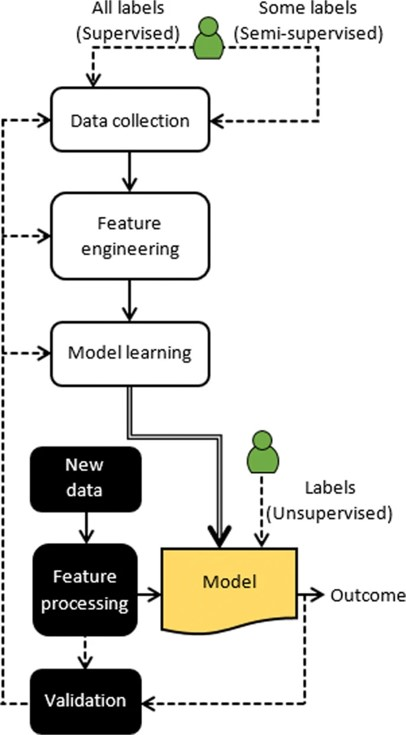
\includegraphics[scale=.8]{./figures/Solution}
\caption{اجزاء سازنده‌ی راه حل‌های مبتنی بر یادگیری ماشین}\label{fig.1}
\end{figure}

\newpage

\section{الگوهای یادگیری}

در یادگیری ماشین چهار الگوی یادگیری وجود دارد، این الگوها بر مراحل بعدی تأثیر می‌گذارند. هدف کلی این است که با توجه به برخی از مجموعه‌های داده نتیجه بگیریم. این الگوها برپایه‌ی دو روش فکری مولد  \LTRfootnote{\lr{Generative}}  و متمایزکننده \LTRfootnote{\lr{Discriminative}} هستند که ریشه در قانون بیز  \LTRfootnote{\lr{Bayes’ Theorem}} دارند:

\begin{equation}
    P(A|B) = \frac{P(B|A)*P(A)}{P(B)}
\end{equation}

%$$
%P(A|B) = \frac{P(B|A)*P(A)}{P(B)}
%$$
این چهار الگوی یادگیری عبارتند از:
\begin{itemize}
\item تحت نظارت\LTRfootnote{\lr{Supervised Learning}}: در حل مسائل طبقه‌بندی و رگرسیون کاربرد دارد و از مجموعه داده‌های برچسب‌دار برای مدل کردن استفاده می‌کنند.
\item نیمه نظارت\LTRfootnote{\lr{Semi-supervised Learning}}: اگر برچسب‌ها ناقص باشند از یادگیری نیمه نظارتی استفاده می‌شود.
\item بدون نظارت\LTRfootnote{\lr{Unsupervised Learning}}: اگر داده‌ها بی‌برچسب باشند از یادگیری بدون نظارت استفاده خواهد شد. از این روش بیشتر در مسائل خوشه بندی استفاده می‌شود.
\item تقویتی\LTRfootnote{\lr{Reinforcement Learning(RL)}}: یک فرایند تکراری مبتنی بر عامل است. عامل در محیط به کاوش می‌پردازد و درنهایت آن را بر اساس اعمالش تشویق و یا جریمه می‌کند. درواقع مجموعه داده‌ها شامل همین تشویق و جریمه‌ها می‌باشند. همچنین با دریافت بازخورد از محیط، کاوش‌های بعدی را تعیین می‌شود.
\end{itemize}



\newpage


\section{جمع‌آوری داده}

تکنیک‌های یادگیری ماشین برای ساخت یک مدل موثر یادگیری ماشین برای یک مشکل خاص، نیاز به داده دارند. جمع آوری داده‌ها یک مرحله مهم است، زیرا داده‌ها نه تنها از یک مسئله به مسئله دیگر بلکه در دوره‌های زمانی نیز باهم متفاوت هستند. به طور کلی جمع آوری داده در دو فاز انجام میشود:
\begin{itemize}
\item آفلاین: این امکان را به ما می‌دهد تا داده‌های مربوط به گذشته برای آموزش و تست مدل به کار روند.
\item آنلاین: این امکان را به ما می‌دهد تا داده‌های شبکه در زمان حال برای بازخورد و ورودی برای آموزش مجدد به کار روند.
\end{itemize}

یک منبع برای جمع آوری داده در هر دوفاز استفاده از ابزارهای نظارتی و اندازه گیری، در سطح شبکه است که میتواند به صورت‌های زیر باشد:

\begin{itemize}
\item نظارت فعال: ترافیک اندازه گیری را تزریق می‌کند، مانند بسته‌های پروب \LTRfootnote{\lr{Probe}} در شبکه و داده‌های مربوطه را از این ترافیک جمع آوری می‌کند.
\item نظارت غیرفعال: با مشاهده میزان واقعی ترافیک شبکه، داده‌ها را جمع آوری می‌کند.
\end{itemize}

نظارت فعال به دلیل مصرف پهنای باند از ترافیک تزریقی، هزینه اضافی را به دنبال دارد. در حالیکه، نظارت غیرفعال با هزینه دستگاه‌های اضافی که ترافیک شبکه را برای جمع آوری اطلاعات مربوطه تجزیه و تحلیل می‌کنند، این سربار را از بین می‌برد\cite{ boutaba2018comprehensive}.
\\
پس از جمع آوری داده‌ها، آنها به مجموعه‌های آموزش، اعتبار سنجی و آزمون تجزیه می‌شوند. مجموعه آموزش برای یافتن پارامترهای ایده آل، مجموعه اعتبار سنجی برای انتخاب معماری مناسب و مجموعه آزمون برای ارزیابی عملکرد بی‌طرفانه مدل انتخاب شده استفاده می‌شود. اینکه چه درصدی از داده‌ها را به کدام مجموعه اختصاص دهیم باید با توجه به کلاس‌های مورد علاقه صورت گیرد.
\newpage

\section{مهندسی ویژگی}



داده‌های خام جمع آوری شده ممکن است اضافی یا ناقص باشند. قبل از استفاده از داده‌ها برای یادگیری، باید مرحله قبل از پردازش را طی کرد. مرحله مهم دیگر قبل از یادگیری، یا آموزش یک مدل، استخراج ویژگی است.


مهندسی ویژگی یک جنبه حیاتی در یادگیری ماشین است که شامل انتخاب و استخراج ویژگی است. برای کاهش ابعاد در داده‌های حجیم و شناسایی ویژگی‌های متمایز که سربار محاسباتی را کاهش می‌دهد استفاده می‌شود. استخراج ویژگی‌ها معمولاً یک فرآیند محاسباتی فشرده است که با استفاده از تکنیک‌هایی مانند آنتروپی و تبدیل فوریه از ویژگی‌های موجود می‌توان ویژگی‌های جدیدی را به دست آورد\cite{ boutaba2018comprehensive}.


\section{ایجاد حقیقت عینی}


ایجاد حقیقت عینی درواقع دادن توصیف رسمی (به عنوان مثال برچسب) به کلاس‌های مورد علاقه است. حقیقت عینی دقت مدل‌های یادگیری ماشین را به همراه دارد. همچنین وابستگی متقابل بین داده‌های آموزشی یک کلاس مورد علاقه به کلاس دیگر وجود دارد که بر عملکرد مدل تأثیر می گذارد. عدم تعادل در تعداد داده‌های آموزش در بین کلاس ها، فرضیاتی را که بسیاری از تکنیک‌های یادگیری ماشین دارند، نقض میکند. بنابر این با استفاده از انواع روش‌های نمونه برداری باید تعادل را برقرار کرد\cite{ boutaba2018comprehensive}.



\section{شاخص‌های عملکرد و اعتبارسنجی مدل}

هنگامی که یک مدل یادگیری ماشین ساخته شد و حقیقت عینی مشخص شد، ارزیابی عملکرد مدل یادگیری ماشین که نتایج را توصیف، پیش بینی یا ارزیابی می‌کند، بسیار مهم است. همچنین، باید توجه کنیم که هیچ راهی برای تشخیص الگوریتم یادگیری به عنوان بهترین الگوریتم وجود ندارد و مقایسه میزان خطا در طیف وسیعی از برنامه‌ها عادلانه نیست. از معیارهای عملکرد می‌توان برای اندازه گیری جنبه‌های مختلف مدل مانند قابلیت اطمینان، استحکام، دقت و پیچیدگی استفاده کرد.

%\section{تکامل روش‌های یادگیری ماشین}

\newpage

\section{خلاصه}


در این فصل، روشي كلي براي ساختن راه حل هاي مبتني بر يادگيري ماشين را ارائه دادیم. در ابتدا، انواع الگوهای یادگیری تحت نظارت، نیمه نظارت، بدون نظارت و تقویتی را دیدیم. سپس مرحله جمع آوری داده ها وجود دارد که به صورت آفلاین و آنلاین انجام می‌شود. سپس به سراغ استخراج ویژگی‌ها رفتیم که برای جلوگیری از سربار محاسباتی مرحله‌ای مهم است. بعد از آن ایجاد حقیقت عینی را دیدیم که می‌بایست به نحوی انجام بشود که تعادل در تعداد داده‌های آموزش برقرار شود. و در مرحله آخر می‌بایست مدل تولید شده را مورد اعتبارسنجی و ارزیابی قرار داد.


%\chapter{سیر تحول و کاربرد یادگیری ماشین}

\section{مهندسی ترافیک}
\subsection{پیش بینی ترافیک}

به عنوان یک مسئله مهم تحقیقاتی، تخمین دقیق میزان ترافیک برای کنترل ازدحام، تخصیص منابع، مسیریابی شبکه و حتی برنامه های پخش زنده مفید است. عمدتا دو جهت تحقیق بسته به مشاهدات مستقیم و غیر مستفیم وجود دارد:
\begin{itemize}
    \item پیش بینی سری‌های زمانی\LTRfootnote{\lr{Time Series Forecasting(TSF)}}
    \item توموگرافی شبکه\LTRfootnote{\lr{Network Tomography}}
    
\end{itemize}
با این حال، اندازه‌گیری مستقیم میزان ترافیک، به ویژه در یک فضای شبکه با سرعت بالا در مقیاس بزرگ، هزینه‌ی زیادی دارد.


تمرکز بسیاری از مطالعات موجود در کاهش هزینه اندازه‌گیری با استفاده از معیارهای غیرمستقیم و نه فقط استفاده از الگوریتم‌های مختلف یادگیری ماشین است. برای حل این مشکل دو روش وجود دارد.  با جستجوی دانش خاص دامنه و الگوهای داده کشف نشده، تلاش بیشتری برای توسعه الگوریتم‌های پیچیده انجام دهیم. روش دیگر از رویکرد یادگیری عمیق انتها به انتها الهام گرفته است. برخی از اطلاعات به دست آمده را به عنوان ورودی مستقیم درنظر گرفته و ویژگی‌ها را با کمک مدل یادگیری به طور خودکار استخراج می‌کند \cite{wang2017machine}.

\subsection{طبقه‌بندی ترافیک}

طبقه بندی ترافیک به عنوان یک مولفه اساسی عملکرد در مدیریت شبکه و سیستم‌های امنیتی، برنامه‌ها و پروتکل‌های شبکه را با جریان ترافیک نگاشت می‌کند. 

دو روش‌ سنتی طبقه بندی ترافیک، رویکرد مبتنی بر پورت\LTRfootnote{\lr{Port}} و رویکرد مبتنی بر پیلود\LTRfootnote{\lr{PayLoad}} است. رویکرد مبتنی بر پورت به دلیل استفاده مجدد و یا غیر صحیح از پورت، ناکارامد است، از طرفی رویکرد مبتنی بر پیلود مشکلات حریم خصوصی ناشی از بازرسی بسته‌ها را دارد، که حتی می‌تواند در حضور ترافیک رمزگذاری شده ناکارامد باشد.

\newpage

در نتیجه، رویکردهای یادگیری ماشین بر اساس ویژگی‌های آماری در سال‌های اخیر به ویژه در حوزه امنیت شبکه به طور گسترده مورد بررسی قرار گرفته است. با این حال، تقریبا نمی‌توان که یادگیری ماشین را به عنوان یک راه حل کامل در نظر بگیریم و آن را در یک محیط عملیاتی دنیای واقعی بکار ببریم. زیرا با طبقه بندی غلط در زمینه امنیت شبکه هزینه زیادی ایجاد می کند. به طور کلی، این مطالعات از سناریوهای شناخته‌شده طبقه بندی شروع می‌شود و تا شرایط دنیای واقعی با ترافیک ناشناخته (به عنوان مثال، ترافیک روز صفر\LTRfootnote{\lr{Zeroday}}) ادامه می‌یابد. این فرایند مطالعه بسیار شبیه به فرایند یادگیری ماشین است که از یادگیری تحت نظارت به یادگیری بدون نظارت و نیمه نظارت تکامل می‌یابد، که می‌تواند به عنوان یک الگوی پیشگام برای وارد کردن یادگیری ماشین در زمینه‌های شبکه تلقی شود.

%\subsection{مسیریابی ترافیک}

\section{کارایی و بهینه‌سازی}
\subsection{کنترل ازدحام}

كنترل ازدحام\LTRfootnote{\lr{Congestion Control}} در شبكه مسئول جریان تعداد بسته‌هاي ورودي به شبكه است. این پایداری شبکه، تعادل در استفاده از منابع و نسبت قابل قبول از دست رفتن بسته را تضمین می‌کند. معماری‌های مختلف شبکه مجموعه مکانیسم‌های کنترل ازدحام خود را به کار می‌گیرند. مشهورترین مکانیزم‌های کنترل ازدحام در پروتکل کنترل انتقال\LTRfootnote{\lr{Transmission Control Protocol(TCP)}} پیاده سازی شده‌اند، زیرا این پروتکل همراه با پروتکل اینترنت\LTRfootnote{\lr{Internet Protocol}} اساس اینترنت فعلی را تشکیل می‌دهند. مکانیزم‌های کنترل ازدحام این پروتکل در سیستم‌های نهایی شبکه کار می‌کنند تا هنگام شناسایی ازدحام، سرعت ارسال بسته را محدود کنند. یکی دیگر از مکانیزم‌های معروف کنترل ازدحام، مدیریت صف است که در داخل گره‌های میانی شبکه (به عنوان مثال سوئیچ‌ها و روترها) برای تکمیل کارکرد این پروتکل عمل می‌کند. پیشرفت‌های کنترل ازدحام در اینترنت و معماری‌های تکاملی شبکه وجود داشته است. با وجود این تلاش‌ها، کاستی‌های مختلفی در زمینه‌هایی مانند طبقه بندی بسته‌های از دست رفته، مدیریت صف و به روزرسانی پنجره ازدحام \LTRfootnote{\lr{CWND}}وجود دارد\cite{boutaba2018comprehensive}.
\newpage




\subsection{مدیریت منابع}
مدیریت منابع شامل کنترل منابع حیاتی شبکه، از جمله پردازنده\LTRfootnote{\lr{CPU}}، حافظه، دیسک، سوئیچ‌ها، روترها، پهنای باند، کانال‌های رادیویی و فرکانس‌های آن است. اینها به طور جمعی یا مستقل برای ارائه خدمات استفاده می‌شوند. ارائه دهندگان خدمات شبکه می‌توانند مقدار مشخصی از منابع را فراهم کنند که تقاضای مورد انتظار برای یک سرویس را تأمین کند. با این حال، پیش بینی تقاضا غیرمعمول نیست، در حالی که تخمین زیاد و بیش از حد منجر زیان شود. بنابراین، یک چالش اساسی در مدیریت منابع، پیش بینی تقاضا و تهیه مجدد منابع به صورت پویا است، به طوری که شبکه در برابر تغییرات تقاضای خدمات مقاوم باشد. با وجود کاربرد گسترده یادگیری ماشین برای پیش بینی و مدیریت منابع در مراکز داده ابری، هنوز هم چالش‌های مختلفی برای شبکه‌های مختلف وجود دارد. در این بررسی، دو نوع چالش را در نظر می‌گیریم\cite{ boutaba2018comprehensive}:
\begin{itemize}
\item کنترل پذیرش\LTRfootnote{\lr{ Admission contro}} یک رویکرد غیر مستقیم برای مدیریت منابع است که نیازی به پیش بینی تقاضا ندارد. هدف در کنترل پذیرش، بهینه سازی استفاده از منابع با نظارت و مدیریت منابع در شبکه است. پذیرش یک درخواست جدید برای ارائه دهنده خدمات شبکه درآمدزایی دارد. با این حال، ممکن است کیفیت خدمات موجود را به دلیل کمبود منابع پایین آید و درآمد خود را از دست بدهد. بنابراین، بین پذیرفتن درخواست های جدید و حفظ کیفیت، یک مصالحه وجود دارد. کنترل پذیرش این چالش را برطرف می‌کند و هدف آن به حداکثر رساندن تعداد درخواست های پذیرفته شده با حفظ کیفیت است.
\item تخصیص منابع\LTRfootnote{\lr{ Resource Allocation}} یک مسئله تصمیم‌گیری است که به طور فعال منابع را مدیریت می‌کند تا یک هدف بلند مدت مانند استفاده از منابع یا درآمد را به حداکثر برساند. چالش اساسی در تخصیص منابع، انطباق منابع برای منافع بلند مدت که غیرقابل پیش بینی هستند. تخصیص منابع نمونه‌ای برای برجسته کردن مزایای یادگیری ماشین است، که می‌تواند تهیه منابع را به روش‌های مختلف یاد گرفته و مدیریت کند.
\end{itemize}

\newpage



\section{امنیت شبکه}

معمول ترین رویکرد امنیتی نظارت بر شبکه برای الگوهای تهدید‌های\LTRfootnote{\lr{Threats}} شناخته شده است. با این حال، شبکه در برابر حملات روز صفر آسیب‌پذیر\LTRfootnote{\lr{Vulnerable}} است. به همین دلیل به اقدامات امنیتی نیاز است و نقش یادگیری ماشین در این راستا به طور گسترده بررسی شده است. 


تلاش‌های موجود، متمرکز بر استفاده از یادگیری ماشین در شناسایی سو استفاده‌ها\LTRfootnote{\lr{Misuse detection}} است که به منظور یادگیری الگوی حمله‌های پیچیده از داده‌های تاریخی و تولید قوانین عمومی است که امکان شناسایی انواع حملات شناخته شده را فراهم می‌کند. همچنین تشخیص ناهنجاری\LTRfootnote{\lr{Anomaly detection}} با استفاده از یادگیری ماشین برای کشف حملات روز صفر بررسی شده است. که شامل یادگیری الگوهای رفتار طبیعی و تشخیص انحراف از وضعیت معمول است.\cite{ayoubi2018machine} 


\section{خلاصه}

در این فصل سیر تحول و کاربرد‌های یادگیری ماشین در زمینه‌های مختلف شبکه را دیدیم. ابتدا در زمینه‌ی مهندسی ترافیک به بحث پیش بینی و طبقه‌بندی ترافیک پرداختیم. و از مشکلات و معضلات روش‌های قدیم و جدید صحبت کردیم. سپس به سراغ زمینه کارایی در شبکه ها رفتیم و درمورد کنترل ازدحام بسته‌ها و مدیریت منابع سخت افزاری بحث کردیم. و درنهایت فصل را با دو کاربرد یادگیری ماشین در زمینه امنیت شبکه خاتمه دادیم.





\newpage
%\chapter{مشخصات یک پایان نامه و گزارش علمی}

اگرچه براي همه انواع نوشته‌ها، مشخصات و ويژگي‌هاي واحد و معيني نمي‌توان ذكر كرد، با اين حال در یک پایان نامه یا گزارش علمی باید نکات و موارد کلی که در این فصل ذکر می‌شود، بطور کامل رعایت شده باشد. 

دقت كنيد كه پس از عنوان فصل بايد حداقل توضیحی کوتاه در مورد موضوع نوشته شود و نمي‌توان مستقيماً بعد از آن عنوان بخش را نوشت و همين طور پس از عناوين بخش‌ها و زيربخش‌ها.(مانند دستورالعمل حاضر)
\section{برخورداری از غنای علمی }

يك پایان نامه بايد پیش از هر چيز به‌لحاظ علمي از غناي لازم برخوردار باشد. يعني هدف و پيام روشني داشته باشد و از پيش‌زمينه علمي، بيان دلايل علمی، ارجاعات مورد نیاز و نتيجه‌گيري شفاف بهره ببرد. 

\section{ارجاع به‌موقع و صحیح به منابع دیگر}
هر جمله‌ای که در یک پایان نامه نوشته می‌شود یا یک جمله کاملاً بدیهی است یا باید دلیل آن بیان شود و یا اینکه باید به منبعی که آن موضوع را نقل یا اثبات کرده، ارجاع داده شود. اگر مطلب يا گفتاري از منبعی عيناً در گزارش نقل مي‌شود، بايد آن مطلب داخل گيومه قرار گيرد و با ذكر ماخذ و شماره صفحه، به آن اشاره گردد.


\section{ساده‌نویسی }
سادگی از ضروريات يك نوشته است. نويسنده بايد ساده، روان و در عين حال شيوا و رسا بنويسد و عبارات مبهم، جملات پيچيده و كلمات نامأنوس در نوشته خود به‌كار نبرد. اگر چه افراط در اين امر نيز، به شيوايي نوشته صدمه مي‌زند. به‌كارگیری لغات و اصطلاحات دشوار و دور از ذهن و عبارات و جملات نامنظم و مبهم موجب ايجاد اشكال در فهم خواننده خواهد شد‌. 

 براي ساده‌نويسي بايد در حد امكان از به‌كارگيری كلمات «مي‌بايست»، «بايستي»، «گرديد»، «بوده باشد» و مانند آنها كه تكلف‌آور، غلط مصطلح و يا غيرشيوا هستند، به‌جای «بايد»، «است»، «شد» و مثل آنها، اجتناب شود‌.‌ همين‌طور، «در‌جهت» نمی‌تواند جايگزين خوبی برای كلمه روانی مثل «برای» باشد‌. ‌كلمات و جملات روان و ساده مي‌توانند اغلب مفاهيم را براحتی منتقل كنند‌.‌
 
دقت در تنظیم بندها (پاراگراف‌ها) نيز كمك شاياني به روانی و سادگی فهم مطلب مي‌كند‌.‌ بندهای طولانی نيز مانند جملات طولانی مي‌توانند خسته‌كننده باشند و خواننده را سردرگم كنند‌.‌ يك بند نبايد کمتر از سه یا چهار سطر یا بيشتر از $10$ تا 15 سطر باشد.‌ 

\section{وحدت موضوع}

نویسنده بايد در سراسر نوشته از اصل موضوع دور نيافتد و تمام بحث‌ها، مثال‌ها و اجزاي نوشته با هماهنگي كامل، پيرامون موضوع اصلي باشد و تاثيري واحد در ذهن خواننده القا كند. 
\section{اختصار}

پایان نامه یا گزارش علمی بايد در حد امكان، مختصر و مفيد باشد و از بحث‌هاي غير ضروري در آن پرهيز شود. نوشتن مطالب ارزشمندي كه هيچ ربطي به موضوع ندارد، فاقد ارزش علمي است.
\section{رعایت نكات دستوري و نشانه‌گذاري}
در سراسر پایان نامه بايد قواعد دستوري رعايت شود و اركان و اجزاي جمله در جاي مناسب خود آورده شود. همچنین رعايت قواعد نشانه‌گذاري سبب مي‌شود كه بيان نويسنده روشن باشد و خواننده به سهولت و با کمترین صرف انرژی مطالب را مطالعه و درك كند.
\section{توجه به معلومات ذهنی مخاطب}
نويسنده بايد همواره مخاطب خود را در برابر خود تصور كند و با توجه به معلومات ذهني مخاطب  تمامي پیش‌نیازهای لازم براي درك مطالب مورد بحث را، از پیش براي مخاطب فراهم كند.

\section{رعایت مراحل اصولی نگارش}
هر کار علمی زمانی به بهترین شکل قابل انجام است که بر اساس یک برنامه‌ریزی مشخص انجام شود. تهیه یک متن علمي با کیفیت نیز نیازمند برنامه‌ریزی مناسب و اجرای منظم آن می‌باشد. مراحل نگارش را عموماً می‌توان به ترتیب زیر درنظر گرفت:
\begin{itemize}


\item	تهيه فهرستی از عناوین اصلي و فرعی که باید نوشته شود
\item 	اولویت‌بندی و تعیین ترتیب منطقی فصل‌ها و بخش‌های گزارش
\item 	گردآوري اطلاعات اولیه راجع به هر بخش و زیربخش
\item 	تدوین مطالب جدیدی که باید به قلم نگارنده به گزارش اضافه شود
\item 	تایپ كردن مطالب با رعایت کامل نکاتی که در این دستورالعمل آموزش داده می‌شود
\end{itemize}
رعایت نظم و ترتیب در اجرای مراحل ذکر شده هم فرآیند تهیه پایان نامه یا گزارش علمی را برای نگارنده آسان می‌کند و هم کیفیت نگارش را به میزان قابل توجهی افزایش می‌دهد.

















%\chapter{نتيجه‌گيري و پیشنهادات}
%%%%%%%%%%%%%%%%%%%%%%%%%%%%%%%%%%%%%%%%%%%
\section{نتیجه‌گیری}
با توجه به ناهمگنی شبکه‌ها، پذیرش تکنیک‌های یادگیری ماشین در حوزه شبکه برای پیشرفت‌های بالقوه ضروری است. با این وجود، عملی کردن آن برای محققان شبکه به دلیل کمبود تجارب مرتبط با یادگیری ماشین، آسان نیست. در این گزارش، یک راهنمایی عملی برای محققان جهت کشف پارادایم‌های جدید یادگیری ماشین برای تحقیقات شبکه در آینده ارائه دادیم. برای درک عمیقتر، آخرین پیشرفت‌های یادگیری ماشین برای شبکه را خلاصه کردیم که چندین روش مهم شبکه را شامل می‌شد، از جمله اندازه گیری، پیش بینی و برنامه ریزی. علاوه بر این، بسیاری از موضوعات مطرح نشدند.

\section{پیشنهادات}
درحالی که آینده همیشه مبهم بوده است اما در این گزارش سعی شد تا مروری بر مباحث یادگیری ماشین و کاربرد آن در شبکه‌های کامپیوتری داشته باشیم. پژوهش‌های بسیاری در این زمینه‌ها شده است. اما این زمینه هنوز نیازمند ایده‌ها و پرورش آنهاست. توصیه می‌شود مبحث پروتکل شبکه خودکار دنبال شود به دلیل آنکه پتانسیل بسیار بالایی هم در زمینه‌ ایده‌پردازی و هم در تحقیقات عملی میتوان داشت.


در آخر از محققان درخواست می‌شود به ایده‌هاي خود گوش بدهند و بدانند که بشر توسط ایده‌هایی پیشرفت کرد که بسیاري آنها را ناممکن می‌دانستند.


%--------------------------------------------------------------------------appendix( مراجع و پیوست ها)
\chapterfont{\vspace*{-2em}\centering\LARGE}%

\appendix
\bibliographystyle{plain-fa}
\bibliography{references}
\chapter*{‌پیوست}
\markboth{پیوست}{}
\addcontentsline{toc}{chapter}{پیوست}
موضوعات مرتبط با متن گزارش پایان نامه كه در يكی از گروه‌های زير قرار می‌گيرد، در بخش پيوست‌ها آورده شوند:
\begin{enumerate}
\item  اثبات های رياضی يا عمليات رياضی طولانی‌.‌
\item داده و اطلاعات نمونه (های) مورد مطالعه (\lr{Case Study}) چنانچه طولانی باشد‌.‌
\item نتايج كارهای ديگران چنانچه نياز به تفصيل باشد‌.‌
\item مجموعه تعاريف متغيرها و پارامترها، چنانچه طولانی بوده و در متن به انجام نرسيده باشد‌.‌
\end{enumerate}
% براي شماره‌گذاري روابط، جداول و اشكال موجود در پيوست‌ از ساختار متفاوتي نسبت به متن اصلي استفاده مي‌شود كه در زير به‌عنوان نمونه نمايش داده شده‌است. 
% \begin{equation}
%F=ma
%\end{equation}
\section*{کد میپل }
\begin{latin}
\begin{verbatim}

with(DifferentialGeometry):
with(Tensor):
DGsetup([x, y, z], M)
																	frame name: M
a := evalDG(D_x)
																	D_x
b := evalDG(-2 y z D_x+2 x D_y/z^3-D_z/z^2)


\end{verbatim}
\end{latin}
%--------------------------------------------------------------------------dictionary(واژه نامه ها)
%اگر مایل به داشتن صفحه واژه‌نامه نیستید، خط زیر را غیر فعال کنید.
%*\parindent=0pt
%*%
\chapter*{واژه‌نامه‌ی فارسی به انگلیسی}
\pagestyle{style9}

\addcontentsline{toc}{chapter}{واژه‌نامه‌ی فارسی به انگلیسی}
%%%%%%
\begin{multicols*}{2}

{\bf آ}
\vspace*{3mm}


\farsiTOenglish{اسکالر}{Scalar}


\vspace*{3mm}
{\bf ب}
\vspace*{3mm}

\farsiTOenglish{بالابر}{Lift}


\vspace*{3mm}
{\bf پ}
%%\vspace*{3mm}

\farsiTOenglish{پایا}{Invariant}



\vspace*{3mm}
{\bf ت}
%%\vspace*{3mm}

\farsiTOenglish{ تناظر }{Correspondence}


\vspace*{3mm}
{\bf ث}
%%\vspace*{3mm}

\farsiTOenglish{ثابت‌ساز}{Stabilizer}

\vspace*{3mm}
{\bf ج}
%%\vspace*{3mm}

\farsiTOenglish{جایگشت}{Permutation}



\vspace*{3mm}
{\bf چ}
%%\vspace*{3mm}


\farsiTOenglish{چند جمله‌ای }{Polynomial}

\vspace*{3mm}
{\bf ح}
%%\vspace*{3mm}

\farsiTOenglish{حاصل‌ضرب دکارتی}{Cartesian product}


\vspace*{3mm}
{\bf خ}
%%\vspace*{3mm}

\farsiTOenglish{خودریختی}{Automorphism}

\vspace*{3mm}
{\bf د}
%%\vspace*{3mm}

\farsiTOenglish{درجه}{Degree}


\vspace*{3mm}
{\bf ر}
%%\vspace*{3mm}


\farsiTOenglish{ریزپردازنده}{microprocessor}


\vspace*{3mm}
{\bf ز}
%%\vspace*{3mm}


\farsiTOenglish{زیرمدول}{Submodule}


\vspace*{3mm}
{\bf س}
%%\vspace*{3mm}

\farsiTOenglish{سرشت}{Character}


\vspace*{3mm}
{\bf ص}
%%\vspace*{3mm}

\farsiTOenglish{صادقانه}{Faithful}

\vspace*{3mm}
{\bf ض}
%%\vspace*{3mm}

\farsiTOenglish{ضرب داخلی}{Inner product}

\vspace*{3mm}
{\bf ط}
%%\vspace*{3mm}


\farsiTOenglish{طوقه}{Loop}


\vspace*{3mm}
{\bf ظ}
%%\vspace*{3mm}


\farsiTOenglish{ظرفیت}{Valency}
 
\vspace*{3mm}
{\bf ع}
%%\vspace*{3mm}


\farsiTOenglish{عدم مجاورت}{Nonadjacency}



\vspace*{3mm}
{\bf ف}
%%\vspace*{3mm}

\farsiTOenglish{فضای برداری}{Vector space}



\vspace*{3mm}
{\bf ک}
%%\vspace*{3mm}

\farsiTOenglish{کاملاً تحویل‌پذیر}{Complete reducibility}


\vspace*{3mm}
{\bf گ}
%%\vspace*{3mm}


\farsiTOenglish{گراف}{Graph}



\vspace*{3mm}
{\bf م}
%%\vspace*{3mm}

\farsiTOenglish{ماتریس جایگشتی}{Permutation matrix }


\vspace*{3mm}
{\bf ن}
%%\vspace*{3mm}

\farsiTOenglish{ناهمبند}{Disconnected}


\vspace*{3mm}
{\bf و}
%%\vspace*{3mm}

\farsiTOenglish{وارون‌پذیر}{Invertible}


\vspace*{3mm}
{\bf ه}
%%\vspace*{3mm}

\farsiTOenglish{همبند}{Connected}



\vspace*{3mm}
{\bf ی}
%%\vspace*{3mm}

\farsiTOenglish{یال}{Edge}




\end{multicols*}%
%*%%%%%%
\chapter*{ واژه‌نامه‌ی انگلیسی به فارسی}
\pagestyle{style9}
\lhead{\thepage}\rhead{واژه‌نامه‌ی انگلیسی به فارسی}
\addcontentsline{toc}{chapter}{واژه‌نامه‌ی انگلیسی به فارسی}

\LTRmulticolcolumns
\begin{multicols}{2}
{\hfill\bf  \lr{A}}
%%\vspace*{1.5mm}

\englishTOfarsi{Automorphism}{خودریختی}

\vspace*{3mm}
{\hfill\bf   \lr{B}}
%%\vspace*{1.5mm}

\englishTOfarsi{Bijection}{دوسویی}

\vspace*{3mm}
{\hfill\bf   \lr{C}}
%%\vspace*{1.5mm}

\englishTOfarsi{Cycle group}{گروه دوری}

\vspace*{3mm}
{\hfill\bf   \lr{D}}
%%\vspace*{1.5mm}

\englishTOfarsi{Degree}{درجه}

\vspace*{3mm}
{\hfill\bf   \lr{E}}
%%\vspace*{1.5mm}

\englishTOfarsi{Edge}{یال}

\vspace*{3mm}
{\hfill\bf   \lr{F}}
%%\vspace*{1.5mm}

\englishTOfarsi{Function}{تابع}

\vspace*{3mm}
{\hfill\bf   \lr{G}}
%%\vspace*{1.5mm}

\englishTOfarsi{Group}{گروه}

\vspace*{3mm}
{\hfill\bf   \lr{H}}
%%\vspace*{1.5mm}

\englishTOfarsi{Homomorphism}{همریختی}

\vspace*{3mm}
{\hfill\bf   \lr{I}}
%%\vspace*{1.5mm}

\englishTOfarsi{Invariant}{پایا}

\vspace*{3mm}
{\hfill\bf   \lr{L}}
%%\vspace*{1.5mm}

\englishTOfarsi{Lift}{بالابر}

\vspace*{3mm}
{\hfill\bf   \lr{M}}
%%\vspace*{1.5mm}

\englishTOfarsi{Module}{مدول}

\vspace*{3mm}
{\hfill\bf   \lr{N}}
%%\vspace*{1.5mm}

\englishTOfarsi{Natural map}{نگاشت طبیعی}

\vspace*{3mm}
{\hfill\bf   \lr{O}}
%%\vspace*{1.5mm}

\englishTOfarsi{One to One}{یک به یک}

\vspace*{3mm}
{\hfill\bf   \lr{P}}
%%\vspace*{1.5mm}

\englishTOfarsi{Permutation group}{گروه جایگشتی}

\vspace*{3mm}
{\hfill\bf   \lr{Q}}
%%\vspace*{1.5mm}

\englishTOfarsi{Quotient graph}{گراف خارج‌قسمتی}

 \vspace*{3mm}
{\hfill\bf   \lr{R}}
%%\vspace*{1.5mm}

\englishTOfarsi{Reducible}{تحویل پذیر}

\vspace*{3mm}
{\hfill\bf   \lr{S}}
%%\vspace*{1.5mm}

\englishTOfarsi{Sequence}{دنباله}

 \vspace*{3mm}
{\hfill\bf   \lr{T}}
%%\vspace*{1.5mm}

\englishTOfarsi{Trivial character}{سرشت بدیهی}

\vspace*{3mm}
{\hfill\bf   \lr{U}}
%%\vspace*{1.5mm}

\englishTOfarsi{Unique}{منحصربفرد}

\vspace*{3mm}
{\hfill\bf   \lr{V}}
%%\vspace*{1.5mm}

\englishTOfarsi{Vector space}{فضای برداری}
\end{multicols}
%--------------------------------------------------------------------------index(نمایه)
%اگر مایل به داشتن صفحه نمایه نیستید، خط زیر را غیر فعال کنید.
\pagestyle{style7}
\printindex
\pagestyle{style7}
%*%کلمات کلیدی انگلیسی
\latinkeywords{Write a 3 to 5 KeyWords is essential. Example: AUT, M.Sc., Ph. D,..}
%چکیده انگلیسی

\en-abstract{
This page is accurate translation from Persian abstract into English.
}
%%%%%%%%%%%%%%%%%%%%% کدهای زیر را تغییر ندهید.

\newpage
\thispagestyle{empty}
\begin{latin}
\section*{\LARGE\centering Abstract}

\een-abstract

\vspace*{.5cm}
{\large\textbf{Key Words:}}\par
\vspace*{.5cm}
\elatinkeywords
\end{latin}
%*% در این فایل، عنوان پایان‌نامه، مشخصات خود و چکیده پایان‌نامه را به انگلیسی، وارد کنید.
%%%%%%%%%%%%%%%%%%%%%%%%%%%%%%%%%%%%
\baselineskip=.6cm
\begin{latin}

\latinfaculty{Department of ...}


\latintitle{Title of Thesis}


\firstlatinsupervisor{Dr. }

%\secondlatinsupervisor{Second Supervisor}

\firstlatinadvisor{Dr. }

%\secondlatinadvisor{Second Advisor}

\latinname{Name}

\latinsurname{Surname}

\latinthesisdate{Month \& Year}

\latinvtitle
\end{latin}

\end{document}